\clearpage
\section{Activity Diagram Design}

\subsection{Workflow Description}

The activity diagram models the operational workflow of the Decentralized Smart Power Grid System from meter data collection to dashboard updates.
\subsection{Activity Diagram}
Figure~\ref{fig:activity} presents the activity flow.

\begin{figure}[H]
    \centering
    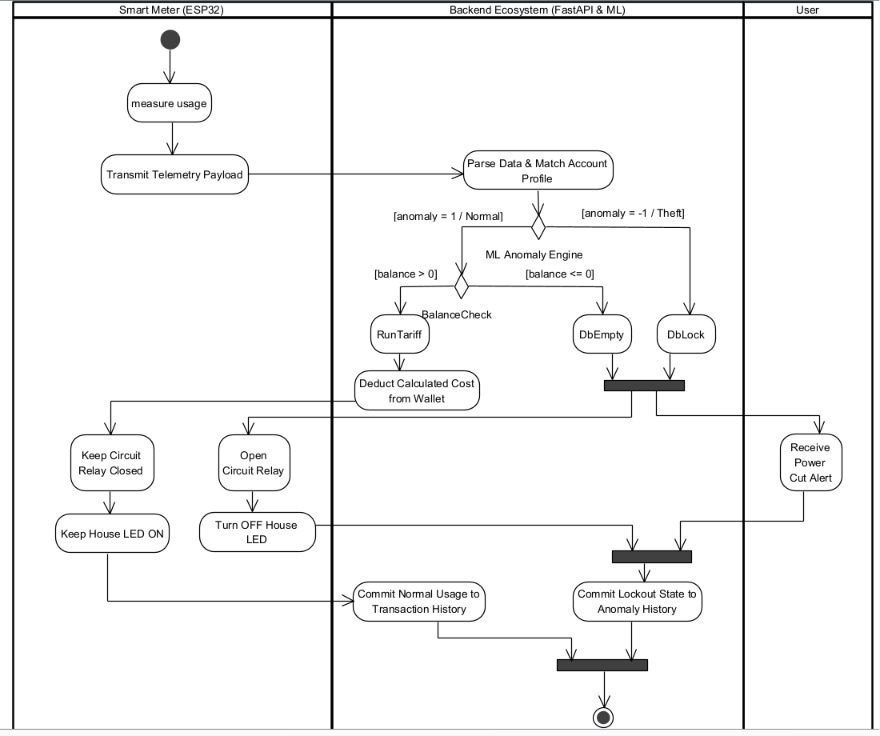
\includegraphics[width=0.85\textwidth]{graphics/activity.jpeg}
    \caption{Activity Diagram of the Decentralized Smart Power Grid System}
    \label{fig:activity}
\end{figure}

\subsection{Workflow Explanation}

The workflow begins with collecting energy consumption data from the smart meter. The backend validates the incoming telemetry, executes blockchain-based prepaid billing, performs anomaly detection, updates system records, and finally displays the latest information through the dashboard.